
\clearpage
\section{The Memory System}

\subsection{The Cache Structure}

Each cache structure consists of the cache and multiple
queues. Figure~\ref{fig:cache} shows the overall cache structure in
the \SIM. There are two flows: 1) cache access flow: from a processor
or upper level cache miss, try to access the cache and 2) cache fill
flow: in case of a cache miss, the data is supplied from the lower
level cache or DRAM. Section~\ref{sec:queue} details all queues and
Section~\ref{sec:cache-flow} describes the flows between queues and a
cache.

\begin{figure*}[htb]
\centering
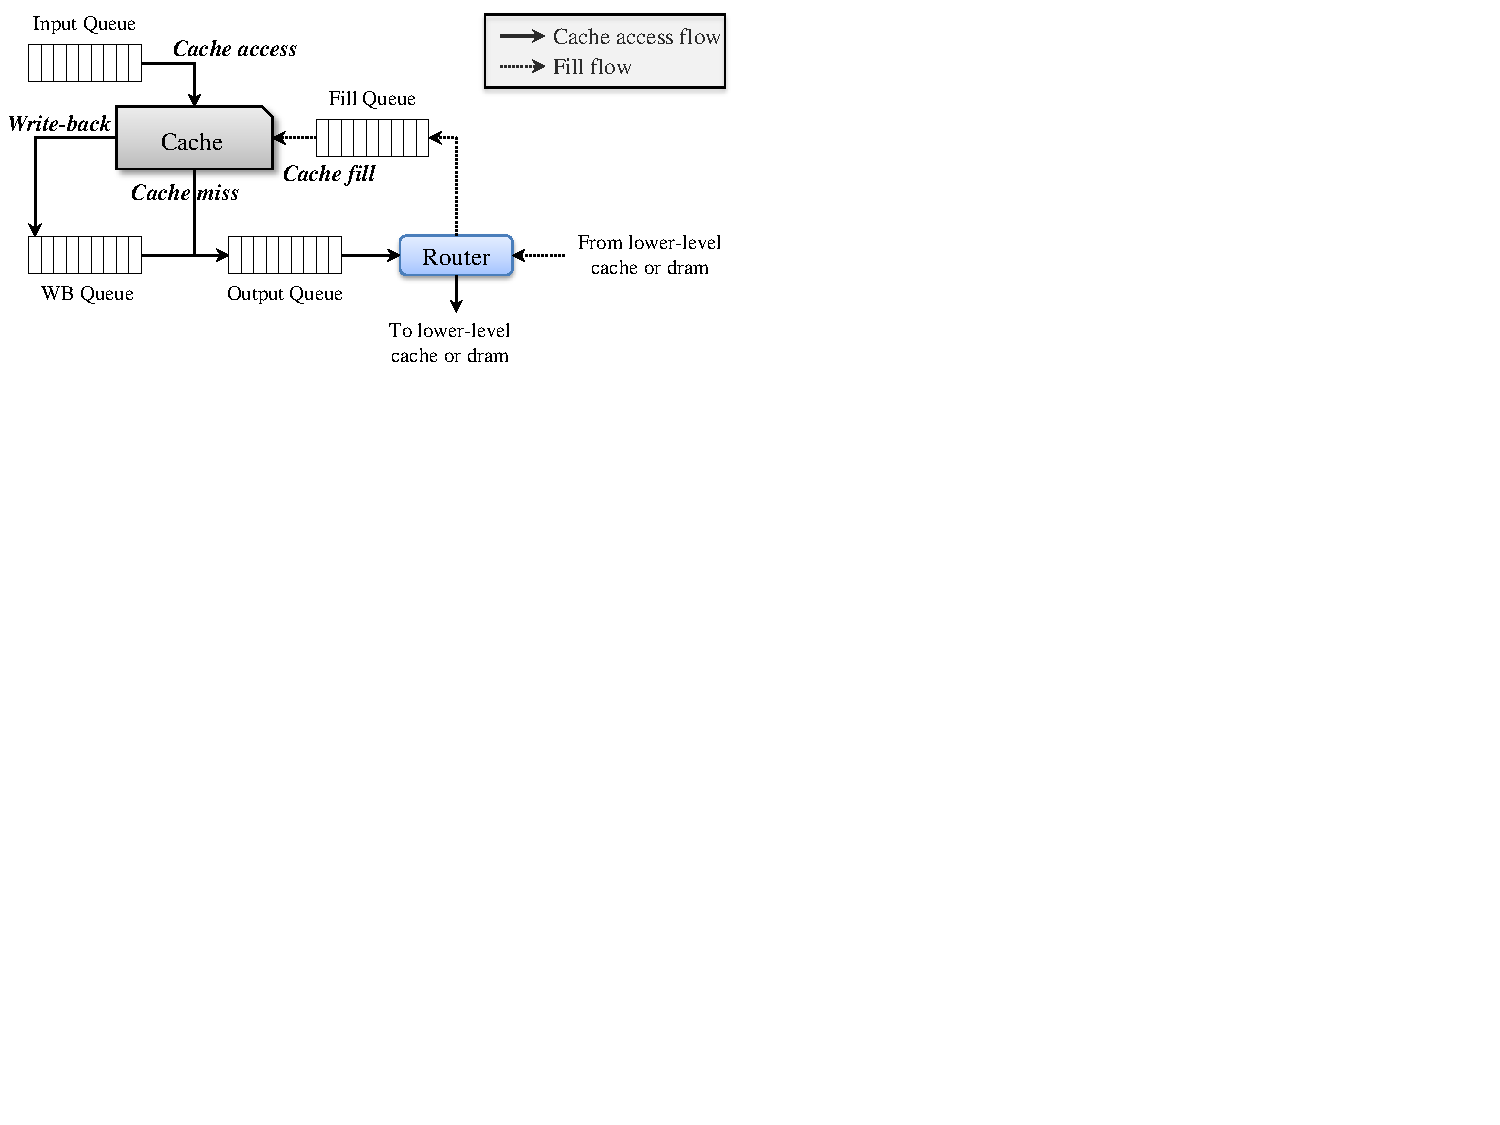
\includegraphics{fig/cache}
\caption{The cache structure.}
\label{fig:cache}
\end{figure*}


\subsubsection{The Queues}
\label{sec:queue}

All cache accesses flow from one queue to the other queue. 

\begin{itemize}
  \item input queue - to access a cache. Requests due to upper-level
  cache misses are inserted in this queue.

  \item output queue - as a result of a cache-miss, a request will be
  inserted into the output queue to be supplied data from the
  lower-level caches or DRAM.

  \item write-back queue - In \SIM, we model write-back caches. When a
  cache line is evicted and dirty, this line needs to be written back
  in the lower level. All write-back requests are initially inserted
  into the write-back queue.

  \item fill queue - requests in this queue tries to fill the data
  that is returned from the lower-level cache or DRAM.

  \item coherence queue - this queue is intended for handling
  coherence traffics, but this is currently not modeled.
\end{itemize}


\subsubsection{The Flows in the Cache Structure}
\label{sec:cache-flow}

\begin{itemize}

  \item Upper-level cache to input queue : upper-level cache miss

  \item input queue to cache : access the cache

  \item cache to output queue : cache miss and lower-level cache access

  \item cache to write-back queue : write-back requests

  \item write-back queue to output queue : to access lower-level cache

  \item output queue to the router : to access the lower-level cache
  through the on-chip interconnection network.

  \item router to the fill queue : the data from the lower-level cache
  or DRAM

\end{itemize}


\subsection{The Hierarchy}

\SIM maintains very flexible memory hierarchy.

